\documentclass[a4paper]{report}
\usepackage[left=3cm, right=3cm]{geometry}
\usepackage{lipsum}
\usepackage{tikzpagenodes}
\usepackage{pgfplots}
\usepackage{tikz}
\usepackage{graphicx}
\usepackage{tikz-3dplot}
\usetikzlibrary{arrows,decorations.pathmorphing,backgrounds,positioning,fit,matrix}
\pgfplotsset{compat=1.8}
\usepackage{graphics} % for pdf, bitmapped graphics files
\usepackage{epsfig} % for postscript graphics files
\usepackage[colorlinks=true,citecolor=green]{hyperref}
\usepackage{cite}
\usepackage{amsmath,amssymb,amsfonts}
\usepackage{algorithmic}
\usepackage{graphicx}
\usepackage{url}
\usepackage{cite}
\usepackage{bm}
\usepackage{pbox}
\usepackage{siunitx,booktabs,etoolbox}
\usepackage{ulem}

%\usepackage{pgf,tikz,pgfplots}
%\pgfplotsset{compat=1.15}
%\usepackage{mathrsfs}

\usetikzlibrary{arrows}

\def\BibTeX{{\rm B\kern-.05em{\sc i\kern-.025em b}\kern-.08em
    T\kern-.1667em\lower.7ex\hbox{E}\kern-.125emX}}

\begin{document}
\title{Pose Estimation}
\author{Xiao Hu, emails: \url{xiahaa@space.dtu.dk}}
\maketitle
\tableofcontents
\chapter{$3$D to $3$D case}
\begin{figure}
	\centering
	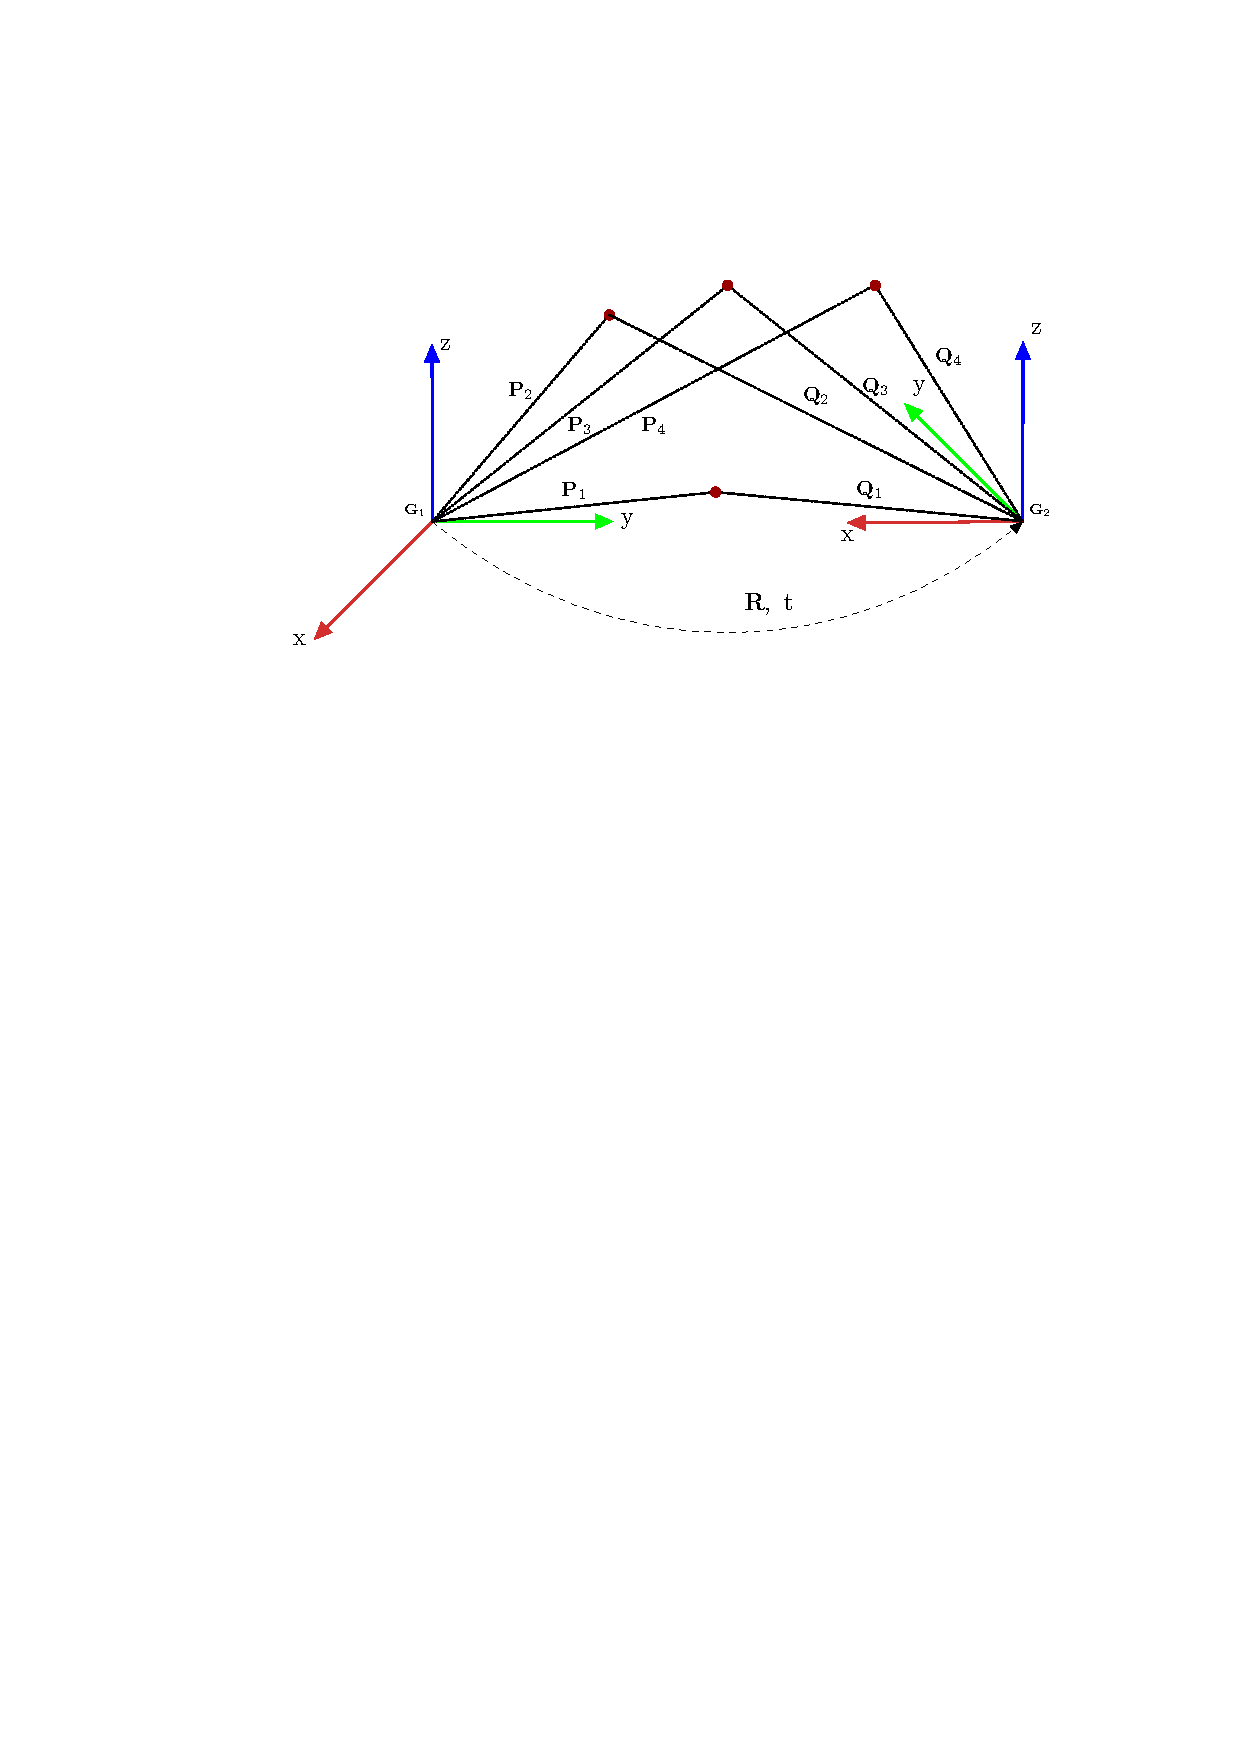
\includegraphics[scale=0.8]{hand_eye_files/vision/figures/p3.pdf}
	\caption{Principles of the $3$D to $3$D pose estimation problem.}
\end{figure}
\section{Problem Formulation}
Let $\mathbf{P}_i$ and $\mathbf{Q}_i$ ($i=1,\ 2,\ ,\ \cdots,\ n$) be two sets of corresponding points in $\mathbb{R}^{3}$. The aim is to find a rigid transformation that align optimally the two sets in the least square sense:
$$
\mathbf{R,t}=\underset{\mathbf{R}\in \mathbb{SO}(3),\ \mathbf{t} \in \mathbb{R}^3}{argmin} \underbrace{\sum_{i=1}^{n} w_i||\mathbf{RP}_i+\mathbf{t}-\mathbf{Q}_i||^2}_{E}
$$
where $w_i$ denotes the corresponding weight for each point pair. 

\section{Solution}
The following introduced solutions were documented in~\cite{sorkine2017least}.

\subsection{SVD}
\paragraph{Translation} It is to see that the objective function is defined in a quadratic form on $\mathbf{t}$. Consequently, if we assume $\mathbf{R}$ is known, $\mathbf{t}$ can be easily found by taking the derivative and letting it equal to zero (first-order optimality condition for differentiable function):
\begin{align*}
\frac{\partial E}{\partial \mathbf{t}}=\sum_{i=1}^{n} 2w_i(\mathbf{RP}_i+\mathbf{t}-\mathbf{Q}_i)&=0 \Leftrightarrow \\
\mathbf{R}\underbrace{\frac{\sum_{i=1}^{n} w_i\mathbf{P}_i}{\sum_{i=1}^{n} w_i}}_{\bar{\mathbf{P}}} - \underbrace{\frac{\sum_{i=1}^{n} w_i\mathbf{Q}_i}{\sum_{i=1}^{n} w_i}}_{\bar{\mathbf{Q}}} &= -\mathbf{t} \Leftrightarrow \\ 
\bar{\mathbf{Q}}  - \mathbf{R}\bar{\mathbf{P}} &=\mathbf{t}
\end{align*}
Plug this into the objective function, we will have:
\begin{align*}
E &= \sum_{i=1}^{n} w_i||\mathbf{R}(\mathbf{P}_i-\bar{\mathbf{P}})-(\mathbf{Q}_i-\bar{\mathbf{Q}})||^2 \Leftrightarrow \\ 
E &= \sum_{i=1}^{n} w_i||\mathbf{R}\mathbf{x}_i-\mathbf{y}_i||^2,\ \mathbf{x}_i = \mathbf{P}_i-\bar{\mathbf{P}},\ \mathbf{y}_i =\mathbf{Q}_i-\bar{\mathbf{Q}}
\end{align*}
\paragraph{Rotation}
Expand one element as
\begin{align*}
||\mathbf{R}\mathbf{x}_i-\mathbf{y}_i||^2=(\mathbf{R}\mathbf{x}_i-\mathbf{y}_i)^{T}(\mathbf{R}\mathbf{x}_i-\mathbf{y}_i)=\mathbf{x}_i^T\mathbf{x}_i-2\mathbf{y}_i^T\mathbf{Rx}_i+\mathbf{y}_i^T\mathbf{y}_i
\end{align*}
It can be seen that the first and third terms are constant, so it is equivalent to optimize only the second term
\begin{align*}
\mathbf{R}=\underset{\mathbf{R}\in\mathbb{SO}(3)}{argmax} \underbrace{\sum_{i=1}^{n} w_i\mathbf{y}_i^T\mathbf{Rx}_i}_{E'}
\end{align*}
The new objective function $E'$ can be written as
\begin{align*}
E'=trace(\mathbf{WYRX})=\underbrace{diag(w_i)}_{\mathbf{W}_{n\times n}} \underbrace{\left[
\begin{matrix}
\mathbf{y}_1^T \\
\mathbf{y}_2^T \\
\vdots \\
\mathbf{y}_n^T 
\end{matrix}
\right]}_{\mathbf{Y}_{n \times 3}} \mathbf{R} 
\underbrace{\left[
	\begin{matrix}
	\mathbf{x}_1 & \mathbf{x}_2 & \cdots & \mathbf{x}_n 
	\end{matrix}
	\right]}_{\mathbf{X}_{3 \times n}}
\end{align*}
Recall that $trace{\mathbf{AB}}=trace{\mathbf{BA}}$, so 
$$
E'=trace(\mathbf{WYRX})=trace(\mathbf{RXWY})
$$
Use a new matrix $\mathbf{S}_{3 \times 3}=\mathbf{XWY}$ and take the SVD of as $\mathbf{S}=\mathbf{U\Sigma V}^T$
$$
E'=trace(\mathbf{RS})=trace(\mathbf{RU\Sigma V}^T)=trace(\mathbf{\Sigma V^TRU})
$$
where $\mathbf{V},\ \mathbf{R},\ \mathbf{U}$ are all unitary matrix. So their product is also an unitary matrix. Assuming their product is $\mathbf{M}=[\mathbf{m}_{(:,1)}\ \mathbf{m}_{(:,2)}\ \mathbf{m}_{(:,3)}]$, then we have
$$
\mathbf{m}_{(:,i)}^T\mathbf{m}_{(:,i)} = \sum_{j=1}^{3} m_{ji}^2 = 1 \Rightarrow |m_{ji}|\leq 1
$$
Recall the new objective function
\begin{align*}
\mathbf{R}&=\underset{\mathbf{R}\in\mathbb{SO}(3)}{argmax}\ trace(\mathbf{\Sigma M}) \Leftrightarrow \\
\mathbf{R}&=\underset{\mathbf{R}\in\mathbb{SO}(3)}{argmax}\ \sum_{i} \sigma_i m_{ii}
\end{align*}
In order to maximize this objective function, we need to have $m_{ii}=1$. Then, we have
\begin{align*}
&\mathbf{I}=\mathbf{M}=\mathbf{V^TRU} \Leftrightarrow \\
&\mathbf{R}=\mathbf{VU}^T
\end{align*}
This optimization omits one constraint imposed by $\mathbb{SO}(3)$, i.e. $det(\mathbf{R})=1$, since the result is only an orthogonal matrix, not a special orthogonal matrix. Actually, it could be a rotation matrix or a reflection matrix. In case we find a reflection matrix $det(\mathbf{R})=-1$, we need to recover from this reflection matrix a rotation matrix:
\begin{align*}
\mathbf{R}=\mathbf{V}
\left[
\begin{matrix}
1 & 0 & 0 \\ 0&1&0 \\0&0&det(\mathbf{VU}^T)
\end{matrix}
\right]
\mathbf{U}^T
\end{align*}
This is the best since we only perturbate the smallest singular value.

\paragraph{The algorithm}
\begin{itemize}
	\item find $\bar{\mathbf{P}}$ and $\bar{\mathbf{Q}}$.
	\item form $\mathbf{x},\ \mathbf{y}$.
	\item find optimal $\mathbf{R}$.
	\item find optimal $\mathbf{t}$.
	\item non-linear optimization.
\end{itemize}

\subsection{Quaternion}
This closed-form pose estimation solution using unit-quaternion was firstly proposed in~\cite{horn1987closed}.
\paragraph{Quaternion} 
The left and right matrix of a quaternion $\mathbf{q}=\{w,\ x,\ y,\ z\}=\{w, \mathbf{x}^T\}$ is given as
\begin{align*}
	\mathbf{L_{q}}&=\left[
	\begin{matrix}
	w & -\mathbf{x}^T \\
	\mathbf{x} & w\mathbf{I}+skew(\mathbf{x})
	\end{matrix}
	\right] \\
	\mathbf{R_{q}}&=\left[
	\begin{matrix}
	w & -\mathbf{x}^T \\
	\mathbf{x} & w\mathbf{I}-skew(\mathbf{x})
	\end{matrix}
	\right] \\
	skew(\mathbf{x})&=\
	\left[
	\begin{matrix}
	0 & -z & y \\
	z & 0 & -x \\
	-y & x & 0
	\end{matrix}
	\right]
\end{align*}
By using quaternion, we also have the following property:
$$
\mathbf{pq}\cdot \mathbf{r} = \mathbf{p} \cdot \mathbf{rq^*}
$$
where $\mathbf{q^*}=\{w,\ -x,\ -y,\ -z\}$ is the conjugate quaternion of $\mathbf{q}$.

\paragraph{Rotation}
Similar to the SVD solution, the first two step is also to find $\bar{\mathbf{P}}$, $\bar{\mathbf{Q}}$, $\mathbf{x}$, and $\mathbf{y}$. Then a new objective function is defined as
\begin{align*}
\mathbf{R}=\underset{\mathbf{R}\in \mathbb{SO}(3)}{argmax}\ \sum_{i=1}^{n} \mathbf{y} \cdot \mathbf{Rx}
\end{align*}
This can be seen as an optimization which best align the rays generated by one point pair since the $\cdot()$ operation is to find the projection of one vector to other. Using the corresponding quaternion of $\mathbf{R}$, it can be further written as
\begin{align*}
\mathbf{R}=\underset{\mathbf{R}\in \mathbb{SO}(3)}{argmax}\ \sum_{i=1}^{n} \mathbf{y} \cdot \mathbf{Rx}=\underset{\mathbf{R}\in (\mathbb{SO}(3)}{argmax}\ \sum_{i=1}^{n} \mathbf{qq_{x_i}} \cdot \mathbf{q_{y_i}q} = \underset{\mathbf{R}\in (\mathbb{SO}(3)}{argmax}\  \sum_{i=1}^{n} \mathbf{q}^T\mathbf{R}_{\mathbf{q_{x_i}}}^T\mathbf{L}_{\mathbf{q_{y_i}}}\mathbf{q}
\end{align*}
where $\mathbf{q_x}$ is the corresponding quaternion of $\mathbf{x}$ by making $w=0$. 
We use $\mathbf{N}=\sum_{i=1}^{n}\mathbf{R}_{\mathbf{q_{x_i}}}^T\mathbf{L}_{\mathbf{q_{y_i}}}$ and there is another convenient way of computing $\mathbf{N}$:
\begin{align*}
	\mathbf{M}&=\sum_{i=1}^{n} \mathbf{x_iy_i^T} \\
	\mathbf{M}&=\left[
	\begin{matrix}
	S_{xx} & S_{xy} & S_{xz} \\
	S_{yx} & S_{yy} & S_{yz} \\
	S_{zx} & S_{zy} & S_{zz} 
	\end{matrix}
	\right] \\
	\mathbf{N}=&=\left[
	\begin{matrix}
	S_{xx}+S_{yy}+S_{zz} & S_{yz}-S_{zy} & S_{zx}-S_{xz} & S_{xy}-S_{yx} \\
	S_{yz}-S_{zy} & S_{xx}-S_{yy}-S_{zz} & S_{xy}+S_{yx} & S_{zx}+S_{xz} \\
	S_{zx}-S_{xz} &  S_{xy}+S_{yx} & -S_{xx}+S_{yy}-S_{zz}& S_{yz}+S_{zy} \\
	S_{xy}-S_{yx} & S_{zx}+S_{xz} & S_{yz}+S_{zy} & -S_{xx}-S_{yy}+S_{zz} \\
	\end{matrix}
	\right] 
\end{align*}
Now the objetcive function is in a quadratic form of $\mathbf{q}$. Since $\mathbf{N}$ is symmetric and positive-definite, we apply the Eigen-value decomposition to $\mathbf{N}$, i.e. $\mathbf{N}=\mathbf{U}\mathbf{\Sigma}\mathbf{U}^T$. Let $\mathbf{q}'=\mathbf{U}^T\mathbf{q} \Leftrightarrow \mathbf{q}=\mathbf{U}\mathbf{q}'$, so $\mathbf{q}$ can be seen as a linear combination of the basis spanned by $\mathbf{U}$
$$
\mathbf{q}=\alpha_1 \mathbf{e}_1 + \alpha_2 \mathbf{e}_2+\alpha_3 \mathbf{e}_3+\alpha_4 \mathbf{e}_4
$$ 

\chapter{$3$D to $2$D case}
\begin{figure}
\centering
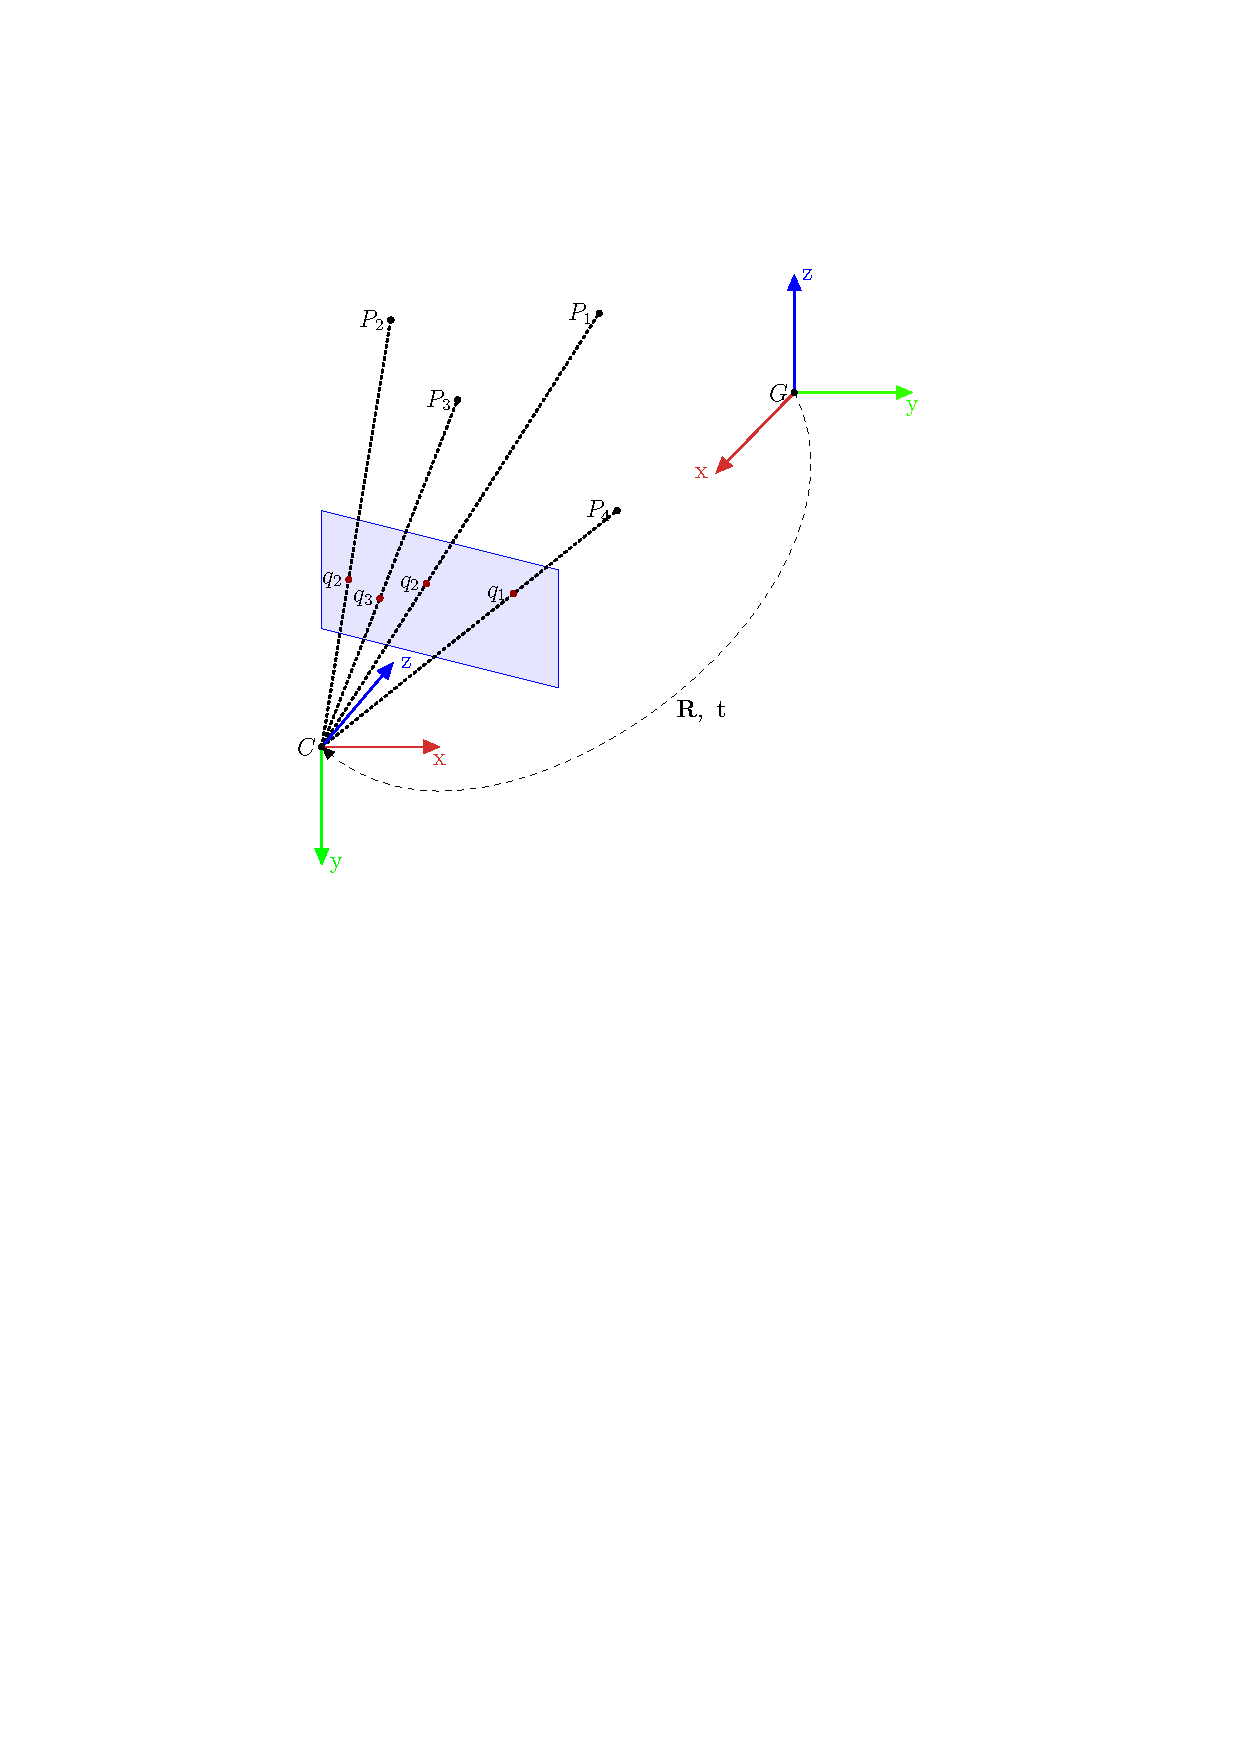
\includegraphics[scale=0.8]{hand_eye_files/vision/figures/pnp.pdf}
\caption{Principles of the Perspective $n$ Point problem.}
\end{figure}
\section{Introduction}
The Perspective-$n$-Point (P$n$P) problem is a fundamental problem in geometric computer vision. Given a certain number ($n$) of correspondences between 3D world points and 2D image measurements, the problem consists of fitting the absolute position and orientation of the camera to the measurement data~\cite{fischler1981random}. A considerable number of approaches have been proposed for the past twenty years. Generally speaking, they can be divided according to different characteristics:
\begin{itemize}
\item By whether or not the solver is run iteratively or not, Iterative V.S. Non-iterative.
\item By the require number of correspondence, P$3$P, P$4$P and more generally, P$n$P.
\end{itemize}

In my opinion, P$3$P and scalable P$n$P would be our focus since other methods are kind of intermediate products of the developing procedure. The reason why P$3$P is still favoured especially after the invention of efficient P$n$P algorithm is as follows:
\begin{itemize}
\item P$3$P is the minimal number of correspondences required to solve the general P$n$P problem. It should be noted that by adding some constraints embedded by the rigid body, this number can go down to $1$, e.g. for non-holonomic vehicle.
\item Although P$n$P algorithm can use the data redundancy to suppress the influence of noises, it can not deal with outliers. The most famous way to deal with outliers is to cascade the P$n$P algorithm with a RANSAC routine. Since for RANSAC, we prefer to use the minimal set to solve a given problem. P$3$P shows its superiority in this sense. 
\end{itemize}
The first P$3$P algorithm in a geometric view is given in~\cite{fischler1981random}, later improvements have been addressed in~\cite{pop00011},~\cite{gao2003complete}, ~\cite{li2011stable} and~\cite{kneip2011novel}.

Scalable P$n$P algorithm means the complexity of the P$n$P algorithm is $\mathcal{O}(n)$, which means its complexity or computational time grows linearly with the number of correspondence. This is very important since we would like to benefit from data redundancy without paying too much cost. The earlier P$n$P algorithms, like~\cite{ansar2003linear} ($\mathcal{O}(n^8)$) and~\cite{quan1999linear} ($\mathcal{O}(n^4)$), are not traceable if we are going to work with thousands of correspondences. EPnP~\cite{lepetit2009epnp}~\cite{moreno2007accurate} is the first P$n$P algorithm with $\mathcal{O}(n)$ complexity, followed by RPnP~\cite{li2012robust}, DLS~\cite{hesch2011direct}~\cite{nakano2015globally}, AsPnP~\cite{zheng2013aspnp}, OPnP~\cite{zheng2013revisiting}, UPnP~\cite{kneip2014upnp}.

Among iterative solutions, LHM~\cite{lu2000fast} is the most famous solution. Other solutions also exist, like RPPnP~\cite{garro2012solving} and the recently published~\cite{8470970}. Iterative solution usually show superior performance under noisy conditions. However, it is easy to see that their computational burden grows at least linearly with the number of correspondences. One of the biggest disadvantage of those iterative solutions is that the global optimality cannot be guaranteed since mathematically speaking, it is a nonlinear optimization problem which is nonconvex.

In this sense, ~\cite{schweighofer2008globally} proposed a method based on Semi-Definite Programming (SDP) and Semi-Definite Relaxation (SDR). Unfortunately, after SDR, the global optimality cannot always be retained to the original problem. Moreover, solving a SDP is usually time-consuming or at least not in real-time.

With regarding to probabilistic optimality, several methods have been proposed to solve this problem in the sense of Maximum-Likelihood Estimation (MLE)~\cite{ferraz2014leveraging},~\cite{urban2016mlpnp}. Currently, I have no plan to detail this kind of solutions. But the principle is to reformulate a cost function in order to maximize the likelihood and then solve this optimization problem iteratively. Also a reasonable estimation of the prior covariance should be built.

Planar case is one of the special case where multiple minimums can exist and hard to distinguish. Similar to~\cite{rpp}, modern approaches may provide more than one solutions if ambiguity exists. This is one point we need to be aware of. The selection of the correct result can be done with the help of other sensors or motion dynamics.

It is also worthy to mention the famous POSIT algorithm which works for object-to-image registration problem~\cite{dementhon1995model}~\cite{oberkampf1996iterative}. It is a iterative algorithm work under the assumption of weak orthogonal projection. An further improvement which allows POSIT works in unknown correspondence condition was published in~\cite{softposit}.

\textcolor{blue}{All those aforementioned algorithms have no capability of dealing with outliers themselves. RANSAC is needed in order to filter out outliers. The conventional routine for outlier removal functions like: 
\begin{itemize}
\item random select a set of correspondences.
\item apply a algorithm and testify the consensus.
\item iterate this until a certain number of iteration or inlier percentage is high enough.
\item refinement with all inliers.
\end{itemize}
This conventional routine is sometimes time-consuming since solving P$n$P and verification (usually based on reprojection error) needs to be carried out in each iteration.}
\textcolor{red}{So this is a still quite open area.} Recent work by~\cite{ferraz2014very} proposes a very fast outlier removal technique. We will detail this in the following section.

Other related topics include: solving P$n$P problem with other intrinsics unknown, such as focus length and radial distortion~\cite{pop00010}~\cite{zheng2016direct}; solving P$n$P problem with even less correspondence with the help of other constraints and sensors~\cite{pylvanainen2009revisiting},~\cite{d2014use},~\cite{d2013use}; continuous solving the P$n$P problem with observers~\cite{pop00016}; over-parameterization~\cite{pop00018}.

\section{Theory and Implementation}
There are two kind of objective functions for the P$n$P problem:

The first one is aiming to minimize the image error or the algebraic error:
\begin{align*}
f =& \underset{\mathbf{R},\ \mathbf{t}}{argmin} \sum_{i=1}^{N}||\mathbf{q}_i-\pi(\mathbf{R}\mathbf{P_i}+\mathbf{t})||^2 \Leftrightarrow \\
 &\underset{\mathbf{R},\ \mathbf{t}}{argmin} \sum_{i=1}^{N}\left((\frac{q_1}{q_3}-\frac{\mathbf{R}_(1,:)\mathbf{P_i}+t_1}{\mathbf{R}_(3,:)\mathbf{P_i}+t_3})^{2}+(\frac{q_2}{q_3}-\frac{\mathbf{R}_(2,:)\mathbf{P_i}+t_2}{\mathbf{R}_(3,:)\mathbf{P_i}+t_3})^{2}
 \right)
\end{align*}
where $\pi$ represents the projective function.

Another function is aiming to minimize the object-space error which is the alignment error of the back-tracing ray of the pixel and the ray from camera center to object points in camera coordinate frame:
\begin{align*}
f =& \underset{\mathbf{R},\ \mathbf{t}}{argmin} \sum_{i=1}^{N}||(\mathbf{I}-\mathbf{V}_i)(\mathbf{R}\mathbf{P_i}+\mathbf{t})||^2,\ with\ \mathbf{V}_i = \frac{\mathbf{q_iq_i}^T}{\mathbf{q_i}^T\mathbf{q_i}}
\end{align*}
\textbf{Note:} we assume here $\mathbf{q}_i$ has been normalized ($\mathbf{q}_i = \mathbf{K}^{-1}\mathbf{q}_i'$).

Generally speaking, the P$n$P problem is to find the answer for the aforementioned two optimization problem. What makes this problem challenging is the rotation matrix $\mathbf{R}\in \mathbb{SO}(3)$ which will implicitly impose nonlinear, nonconvex constraints. This is why the famous Direct-Linear-Transformation (DLT)\footnote{DLT means we omit those constraints and take each elements of $\mathbf{R}$ as separate variables. This can make the objective function as well as the constraints in affine or quadratic form.} method cannot given us a promising result.

Here are some useful techniques which will help us solve this problem~\cite{hartley2007optimal}:
\begin{itemize}
\item Branch-and-Bounding;
\item Convex optimization, such as Second-Order-Cone-Programming (SOCP), SDP: this usually requires relaxation or even solve the prime problem by solving the dual problem;
\item Algebraic Geometry: use Gr\"{o}ebner basis. This is feasible since the objective function and the constraints can be formulate as a polynomial system and the answer is the common root that makes those polynomials vanish~\cite{kukelova2008automatic}. 
\item Manifold Optimization which applies optimization directly on $\mathbb{SO}(3)$ and $\mathbb{SE}(3)$.
\end{itemize}

\subsection{P$3$P}
We start with the P$3$P algorithms. Generally speaking, the P$3$P problem solves this problem by firstly estimating the arc-length of each points in the camera frame, then reconstructs the point cloud in the camera frame by multiplying the arc-length with the back-tracing rays, and finally applies the $3$D to $3$D pose estimation routines in order to find the $\mathbf{R}$ and $\mathbf{t}$.
\begin{figure}
\centering
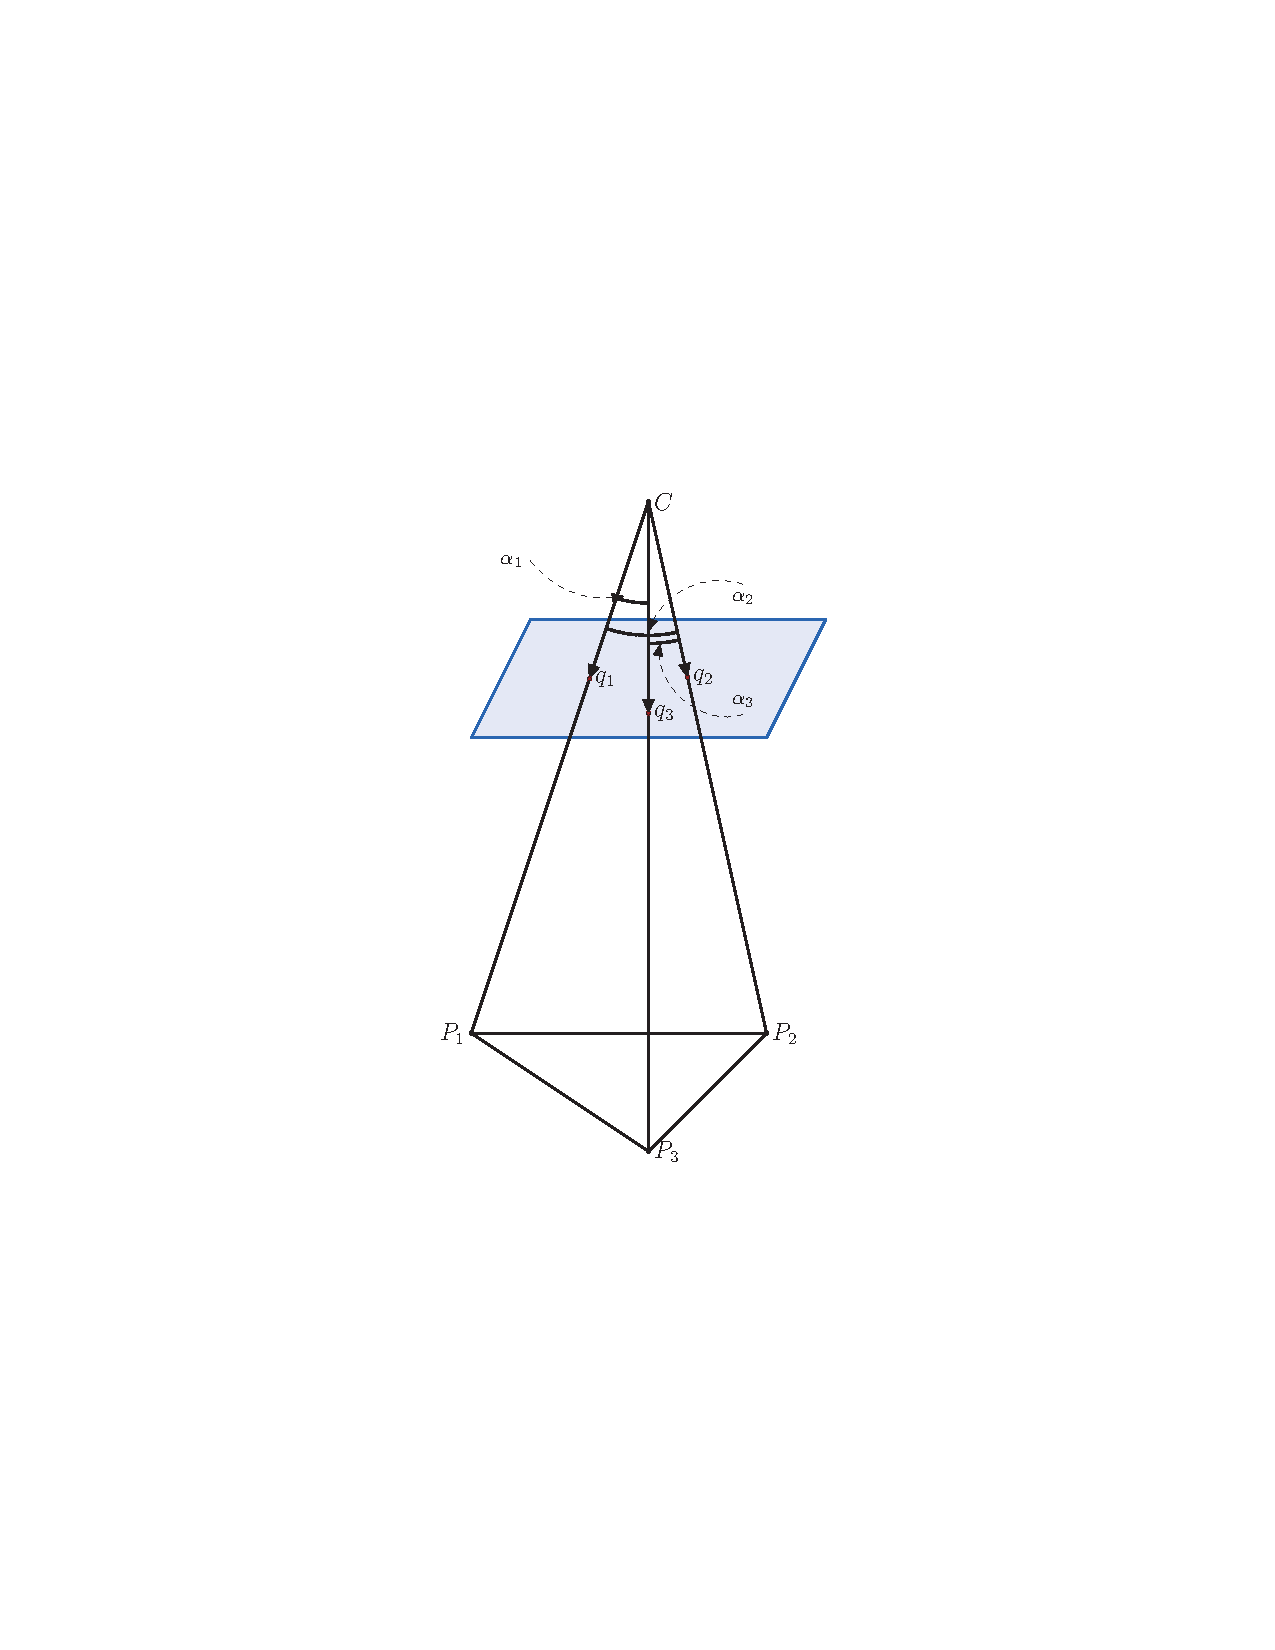
\includegraphics[scale=0.8]{hand_eye_files/vision/figures/p3p.pdf}
\caption{Principles of the Perspective $3$ Point problem.}
\label{fig:p3p}
\end{figure}
\begin{figure}
\centering
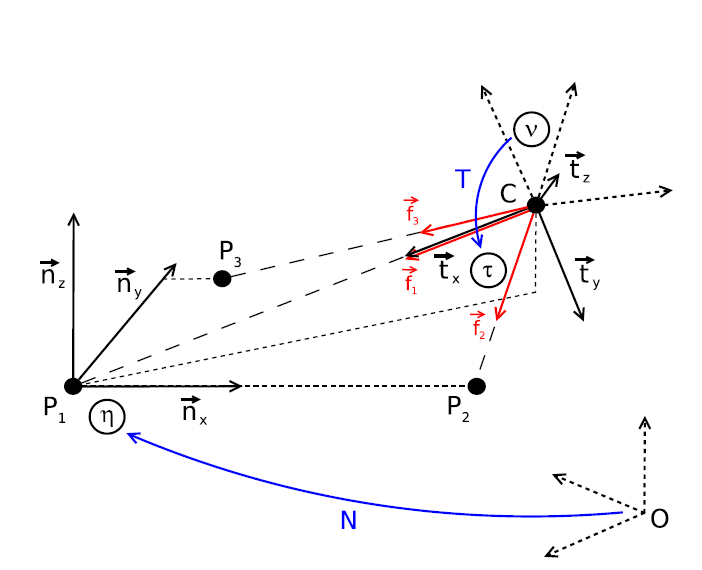
\includegraphics[scale=0.5]{hand_eye_files/vision/figures/p3p_kneip.png}
\caption{Figure from~\cite{kneip2011novel}.}
\label{fig:p3p}
\end{figure}
From Fig~\ref{fig:p3p}, by denoting $|CP_1|=d1,\ |CP_2|=d2,\ |CP_3|=d3,\ |P_1P_2|=d12,\ |P_1P_3|=d13,\ |P_2P_3|=d23,\ $, we will have the following relationship using the cosine rule:
\begin{align*}
d12^2 = d1^2+d2^2-2cos(\alpha_2)d1d2 \\
d13^2 = d1^2+d3^2-2cos(\alpha_1)d1d3 \\
d23^2 = d2^2+d3^2-2cos(\alpha_3)d2d3 \\
\end{align*}
where $\alpha_1 = acos(\mathbf{q}_1 \cdot \mathbf{q}_3),\ \alpha_2 = acos(\mathbf{q}_1 \cdot \mathbf{q}_2),\ \alpha_3 = acos(\mathbf{q}_2 \cdot \mathbf{q}_3)$. By some algebraic operations\footnote{eliminate one variable by the other two and then continue}, we will have a $4^{th}$ order polynomial equation:
\begin{align*}
A_4 t^4+A_3 t^3+A_2 t^2+A_1 t^1+A_0 = 0
\end{align*}
By solving this equation, we will have the arc-length. Continue this for other arcs, we can find them all. By multiplying $\mathbf{q}_i$ with $d_i$, we will have $\mathbf{Q}_i$, then the problem transforms to:
\begin{align*}
f =& \underset{\mathbf{R},\ \mathbf{t}}{argmin} \sum_{i=1}^{N}||\mathbf{Q}_i-\mathbf{R}\mathbf{P_i}+\mathbf{t}||^2
\end{align*}
which is a typical $3$D to $3$D pose estimation problem that can be solved.

P$3$P methods~\cite{fischler1981random},~\cite{gao2003complete}, and~\cite{li2011stable} all function in this way. ~\cite{fischler1981random} is more like a hard-code solution.~\cite{gao2003complete} gives detailed illustration of the P$3$P problem and also their solution under some degenerate cases. However,~\cite{gao2003complete} is too mathematical which is hard to read. But if you only care about the solution, then you can go directly to the normal case.~\cite{li2011stable} is the most clear paper that clearly explain this problem.


The only different P$3$P method was proposed in~\cite{kneip2011novel}. By introducing two intermediate frames, it changes the original $3$D to $2$D problem to a plane problem. After geometric operations, it finally results in a $4^{th}$ order polynomial equation. However, this $4^{th}$ order polynomial does not take arc-length as the variable, but an alternative parameter which represent the tilt angle of the $P_1-P_2-C$ plane. So the final $\mathbf{R},\ \mathbf{t}$ have to be found in another way rather than solving the $3$D to $3$D pose estimation problem. \textcolor{blue}{This method is easy to understand and very fast.}

\subsubsection{Summary of P$3$P}
Here are several points which remains unclear:
\begin{itemize}
\item \textcolor{blue}{which P$3$P gives the best performance in terms of stability, runtime?}
\item \textcolor{blue}{how can P$3$P benefit from data redundancy? Or P$3$P can only be used for outlier removal together with RANSAC?}
\end{itemize}

\subsection{Complex P$n$P}
Here, Complex P$n$P means not-well scalable P$n$P algorithms such as~\cite{quan1999linear} and~\cite{ansar2003linear}. I will begin with~\cite{quan1999linear} and then talk about~\cite{ansar2003linear}.

The linear P$n$P in~\cite{quan1999linear} is based on the cosine rule function we have seen in P$3$P.~\cite{quan1999linear} uses the Sylvester resultant to eliminate variable, which will result in a $8^{th}$ order polynomial which only contains even terms (equals to a $4^{th}$ order polynomial). The idea is quite straightforward: since each tuple-3, e.g ${1,2,3} or {1,4,5}$, will generate a $4^{th}$ order polynomial in, e.g. $d_1$. So, $N$ points generates $C_{N}^{2}$ cosine equations which furthermore generates $\frac{(n-1)(n-2)}{2}$ $4^{th}$ order polynomials (eliminating redundant polynomials). By taking the linearization which means taking $\mathbf{t}=(1,x,x^2,x^3,x^4)^{T}$ as separate terms, we will have a equation like $\mathbf{A}\mathbf{t}=0$. 
$$
\underbrace{
\left[
\begin{matrix}
\mathbf{a}_1 \\
\mathbf{a}_2 \\
\vdots \\
\mathbf{a}_K \\
\end{matrix}
\right]}_{\mathbf{A}}
\left[
\begin{matrix}
1 \\ x \\ x^2 \\ x^3 \\ x^4
\end{matrix}
\right]=\mathbf{0}
$$
Then $\mathbf{t}$ can be found by taking the right singular vector. Supposing the dimension of the null space is over one, which means 
$$
x = \lambda \mathbf{v}_4 + \beta \mathbf{v}_5, \lambda, \beta \in \mathbb{R}.
$$
In order to solve for $\lambda, \beta$, we should use the so-called re-linearization technique:
Notice that $t_it_j=t_kt_l,\ if\ i+j=k+l$, so we call formulate another normal system with $(\lambda^2, \lambda\beta, \beta^2$. We solve again for $\lambda, \beta$ and then for $d_i$. The final pose estimation problem, once again, turns out to be a $3$D to $3$D pose estimation problem. \textcolor{blue}{As can be seen from here, data redundancy is utilized by stacking the $4^{th}$ order polynomial equation and find the null vector. However, since the aforementioned procedure has to be run for each possible arc, for sure, the complexity does not scale very well.}

Another linear P$n$P algorithm is proposed in~\cite{ansar2003linear}. It also starts with the cosine equations. However, they applied linearization as follows:
\begin{align*}
&\text{recall: } x_1^2+x^2-2x_1x_2cos(\alpha_{12})-d_{12}^2=0 \\
&\text{linearization: $\mathbf{t}={x_1^2, x_1x_2, x_2^2}$} \\
&\text{do this for $N$} \Leftrightarrow \\
&\underbrace{
\left[
\begin{matrix}
-2cos(\alpha_{12}) & 0 & \cdots & 0 \\
0 & -2cos(\alpha_{13}) & \cdots & 0 \\
\vdots & \vdots & \ddots & \vdots \\
0 & 0 & \cdots & -2cos(\alpha_{n, n-1})\\
\end{matrix}
\right.
\left|
\begin{matrix}
1 & 1 & 0 & \cdots & 0 & 0 & -d_{12}^2\\
1 & 0 & 1 & \cdots & 0 & 0 & -d_{13}^2\\
\vdots & \vdots & \vdots& \ddots & \ddots & vdots & vdots \\
0 & 0 & \cdots & cdots & 1 & 1 & -d_{n, n-1}^2\\
\end{matrix}
\right]
}_{\mathbf{M}} \\
&\mathbf{M}\mathbf{t} = \mathbf{0}
\end{align*}
Finding $\mathbf{t}$ by choosing the rightmost singular vector and apply a similar relinearization to recover $x$. For $N$ points, we have $C_{N}^2$ cosine equations. Then we have $N$ terms in form of $x_i^2$, $C_{N}^2$ terms in form of $x_ix_j$ and one slack variable $1$. So in total, the solution vector is $\frac{N(N+1)}{2}+1$. The kernel is of dimension $\frac{N(N-1)}{2}$, so we will have a null space of dimension $N+1$. We still needs $\frac{N*N*(N-1)}{2}$ constraints to do the relinearization. As can be seen, this method is extremely complex. The computation time will increase significantly with the number of correspondences. \textcolor{red}{This method is only theoretically meaningful, but cannot be used in practice, especially now we have the $\mathcal{O}(n)$ solutions.}

\subsection{Summary of Complex P$n$P}
The linearization and relinearization techniques opens the gate for later $\mathcal{O}(n)$ P$n$P solutions. Regard to the Complex P$n$P, we could include them as the related work, but use other $\mathcal{O}(n)$ solutions in practice.

\subsection{POSIT \& SoftPOSIT}
\subsubsection{Original POSIT}
POSIT was firstly proposed in~\cite{dementhon1995model} and later refined in~\cite{oberkampf1996iterative} for solving planar case. The original formulation of POSIT is slightly different with the formulation given below. However, the two formulation can be easily transformed by doing some variable replacements. Here I just list the key equations for POSIT algorithm.

The principle of POSIT algorithm is that the perspective projection $\mathbf{x}$ can be corrected by some scales $\epsilon_i$ to match with the scaled orthographic projection $s\mathbf{P}_i$. So we can formulate two normal equations for $\mathbf{x}=[u,\ v]^T$ such as
\begin{align*}
\mathbf{R} &= \left[
\begin{matrix}
\mathbf{i}^T \\ \mathbf{j}^T \\ \mathbf{k}^T
\end{matrix}
\right] \\
s\mathbf{i} &= \mathbf{I},\ s\mathbf{j} = \mathbf{J},\ s\mathbf{k} = \mathbf{K},\\
\mathbf{P}_i \cdot \mathbf{I} &=u_i(1+\epsilon_i)-u_0 \\
\mathbf{P}_i \cdot \mathbf{J} &=v_i(1+\epsilon_i)-v_0 \\
\Leftrightarrow & \\
\mathbf{A}\mathbf{x}&=\mathbf{b}
\end{align*}
By solving $\mathbf{A}\mathbf{x}=\mathbf{b}$ using the pseudo-inverse, we can recover the pose and then update the $\epsilon_i=\frac{\overrightarrow{\mathbf{P}_0\mathbf{P}_i} \cdot \mathbf{k}}{t_z}$. This process iterates until convergence. For planar case, the rank of $\mathbf{A}$ is $2$. Consequently, any solution $x_0$ plus the scaled null vector $\mathbf{x}_{null}$ of $\mathbf{A}$ could be the solution $\mathbf{x}_{0}+\lambda\mathbf{x}_{null}$. We note the solution for $u,\ v$ as $\mathbf{I}_0+\lambda \mathbf{t}_{null}$ and $\mathbf{J}_0+\mu\mathbf{t}_{null}$ (the null vector is the same since $\mathbf{A}$ works both for $u$ and $v$). Then since we know that the correct $\mathbf{I}$ and $\mathbf{J}$ are orthogonal to each other and of the same length:
\begin{align*}
\lambda \mu &= \mathbf{I}_0\mathbf{J}_0 \\
\lambda^2 -\mu^2 &= ||\mathbf{J}_0||^2-||\mathbf{I}_0||^2 \\
\end{align*}
which will results in a $2^{rd}$ polynomial and brings us two solutions. As a result, two possible poses could be returned. As you can see from here, the number of solutions may grow exponentially ($1 \to 2 \to 4 \to 8 \to \cdots$), in order to suppress this curse of dimension,~\cite{oberkampf1996iterative} suggests if over two solutions are generated, only keeps the best two possible solutions. In my experiments, the scheme works well although there is no theoretical proof.
\subsubsection{SoftPOSIT}
SoftPOSIT is an improvement for orginal POSIT algorithm which aims to estimate pose and correspondence simultaneuously. As can be seen from this statement, for SoftPOSIT solution, the correspondence could be unknown or partially known. This serves the biggest difference of SoftPOSIT algorithm relative to other solutions mentioned in this report.
\paragraph{POSIT routine}
Assume object points are  $\mathbf{P}_i,\ i=1,\ \cdots,\ M$ (homogeneous coordiantes) and image points $\mathbf{q}_j,\ j=1,\ \cdots,\ N$ (normalized homogeneous coodrinates, so $f=1$), then the coordinates of object points relative to an origin $\mathbf{P}_0$ can be represented as $\tilde{\mathbf{P}}_i=\mathbf{P}_i-\mathbf{P}_0$. From the perspective projection model, we have:
\begin{align*}
w\left[
\begin{matrix}
x \\ y \\ 1
\end{matrix}\right]&=\left[
\begin{matrix}
\mathbf{R}_{(1,:)}^T & tx \\ 
\mathbf{R}_{(2,:)}^T & ty \\ 
\mathbf{R}_{(3,:)}^T & tz \\ 
\end{matrix}
\right]
\left[
\begin{matrix}
\tilde{\mathbf{P}} \\ 1
\end{matrix}
\right] \\
w\left[
\begin{matrix}
x \\ y 
\end{matrix}\right]&=s
\left[
\begin{matrix}
\mathbf{R}_{(1,:)}^T & tx \\ 
\mathbf{R}_{(2,:)}^T & ty \\ 
\end{matrix}
\right]
\left[
\begin{matrix}
\tilde{\mathbf{P}} \\ 1
\end{matrix}
\right] \\
with\ s=&\frac{1}{t_z},\ w=\frac{\mathbf{R}_{(3,:)}^T\tilde{\mathbf{P}}_i}{tz}+1
\end{align*}
If $t_z >> \mathbf{R}_3^T\tilde{\mathbf{P}}_i$, then $w \approx 1$. Furthermore, we will have 
\begin{align*}
\left[
\begin{matrix}
x \\ y 
\end{matrix}\right]&=s
\left[
\begin{matrix}
\mathbf{R}_{(1,:)}^T & tx \\ 
\mathbf{R}_{(2,:)}^T & ty \\ 
\end{matrix}
\right]
\left[
\begin{matrix}
\tilde{\mathbf{P}} \\ 1
\end{matrix}
\right]
\end{align*}
which defines the scaled orthographic projection. Taking the transpose of this equation, we will have
\begin{align*}
[X,\ Y,\ Z,\ 1]
\underbrace{\left[
\begin{matrix}
s\mathbf{R}_{(1,:)} & s\mathbf{R}_{(2,:)} \\ 
stx & sty \\ 
\end{matrix}
\right]}_{\mathbf{Q}}=[wx,\ wy]
\end{align*}
$\mathbf{Q}$ is the variable we are going to optimize. Once we have $\mathbf{Q}$, we can extract the corresponding blocks as $s\mathbf{R}_{(1,:)}$ and $s\mathbf{R}_{(2,:)}$, since we know that $||\mathbf{R}_1||=1$, $s$ can be recorvered as $s=\sqrt{|s\mathbf{R}_{(1,:)}||s\mathbf{R}_{(2,:)}|}$. Then $\mathbf{R}_{(3,:)}=\mathbf{R}_{(1,:)} \times \mathbf{R}_{(2,:)}$, $t_x = \frac{st_x}{s},\ t_y=\frac{st_y}{s}, t_z=\frac{1}{s}$. This process runs iteratively by firstly letting $w_k=1,\ k=1,\ 2,\ \cdots,\ M$ and update $w_k$ with newly estimated $\mathbf{R}, \mathbf{t}$. The geometric interpretation of this equation is that $w_k$ functions like a correction of the perspective projection $[x,\ y,\ 1]^T$ to the scaled orthographic projection. The overall objective function for POSIT can be written as:
\begin{align*}
E=\sum_{k=1}^{M}\left(
\left(
\mathbf{Q}_1^T \mathbf{P}_k - w_kx_k
\right)^2+
\left(
\mathbf{Q}_2^T \mathbf{P}_k - w_ky_k
\right)^2
\right)
\end{align*}
where $\mathbf{Q}_1=s[\mathbf{R_{(1,:)}}^T \mathbf{tx}]^T$, $\mathbf{Q}_2=s[\mathbf{R_{(2,:)}}^T \mathbf{ty}]^T$, $\mathbf{P}_k=[\tilde{\mathbf{P}}_k^T, 1]^T$. By taking the derivative of $E$ with respect to $\mathbf{Q}_1, \mathbf{Q}_2$, we can get the least-square solution for $\mathbf{Q}_1, \mathbf{Q}_2$ as
\begin{align*}
\mathbf{Q}_1=\left(
\sum_{k=1}\mathbf{P}_k\mathbf{P}_k^T
\right)^{-1}\left(
\sum_{k=1} w_kx_k\mathbf{P}_k
\right) \\
\mathbf{Q}_2=\left(
\sum_{k=1}\mathbf{P}_k\mathbf{P}_k^T
\right)^{-1}\left(
\sum_{k=1} w_ky_k\mathbf{P}_k
\right)
\end{align*}
\paragraph{Correspondence Update routine}
SoftPOSIT~\cite{softposit} algorithm maintains a soft assign matrix $\mathbf{M} \in \mathbb{R}^{M\times N},\ $ (M is the number of object points, and N is the number of the image points) in which the element $m_{ij}$ represents the likelihood of model point $i$ matches with image point $j$. Since we have no information of the correspondence, so for each $w_k$, its correction has to be applied for each image points. Then we compute the pixel distance of each corrected image coordinates with the scaled orthographic projection of the $k^{th}$ object point:
\begin{align*}
d_{kj}^2=(\mathbf{Q}_1\mathbf{P}_k-w_k x_j)^2 + (\mathbf{Q}_2\mathbf{P}_k-w_k y_j)^2
\end{align*}
An threshold $\alpha$ is used as the maximum tolerate distance for considering an correspondence. The modified optimization problem is described as:
\begin{align*}
E=\sum_{k=1}^{M}\sum_{j=1}^{N}m_{kj}\left(
\left(
\mathbf{Q}_1\mathbf{P}_k-w_k x_j
\right)^2+
\left(
\mathbf{Q}_2\mathbf{P}_k-w_k y_j
\right)^2
\right)
\end{align*}
where $m_{kj}$ serves as a weight ($0 \leq m_{kj} \leq 1$). This is a weighted least square problem which can be similarly solved. 

Once we solve for the new pose, we do the update of the soft assign matrix $\mathbf{M}$ by:
\begin{itemize}
	\item compute the matching distance $d_{kj}^2$.
	\item update $w_k=\gamma exp(-\beta(d_{kj}^2-\alpha))$ and truncate this to be within $0-1$.
	\item the row and column of $\mathbf{M}$ should be $1$ since one object point only matches to one image point. So re-normalization is necessary: this is done by alternatively normalize along the row direction and then along the column direction using the so called Sinkhorn algorithm.
\end{itemize}

\subsection{Summary of POSIT \& SoftPOSIT}
SoftPOSIT~\cite{softposit} iterates to solve this problem, which is related to the general expectation-maximization (EM) algorithm. So generally speaking, global optimality is not guaranteed. Secondly, SoftPOSIT algorithm is usually very slow since its working condition is more challenging. From the experiments I have done, SoftPOSIT is not very stable. Sometimes it cannot find the correct solution.


\subsection{Iterative P$n$P}
We will introduce two iterative P$n$P solutions: the LHM~\cite{lu2000fast}, the PP$n$P~\cite{garro2012solving}.
\subsubsection{LHM}
The most famous iterative solution should be~\cite{lu2000fast}. The biggest difference of this method compared with other methods would be classical methods apply optimization using Euler angles which constrain their performance and optimality, while this method does the so-called orthogonal iteration. 

The objective function used in this method is the object-space error:
$$
E = \sum_{i=1}^{N} ||(\mathbf{I}-\mathbf{V}_i)(\mathbf{R}\mathbf{P}_i+\mathbf{t})||^2
$$
It is clear that if we make $\mathbf{R}$ fixed, then the objective function is in the quadratic form of $\mathbf{t}$, which means the optimal $\mathbf{t}$ can be computed as
$$
\mathbf{t}(\mathbf{R})=\frac{1}{N}(\mathbf{I}-\frac{1}{N}\sum_{j}\hat{\mathbf{V}}_j)^{-1} \sum_{j}(\hat{\mathbf{V}}_j-\mathbf{I})\mathbf{R}\mathbf{p}_j
$$
With the equation, the iteration process starts with an initial estimation of the $\mathbf{R}_k$:
\begin{itemize}
	\item compute for the $\mathbf{t}_k$.
	\item compute the transformed point coordiante $\mathbf{q}^k_i=\mathbf{R}_k\mathbf{p}^k_i+\mathbf{t}$.
	\item update $\mathbf{R}_k$ as the minimizer for $\sum_{i=1}^{N}||\mathbf{R}_k\mathbf{p}_i+\mathbf{t}-\hat{\mathbf{V}}_i\mathbf{q}^k_i||^2$, which is a $3$D to $3$D pose estimation problem if we assume $\mathbf{q_i^k}$ is fixed.
	\item iterates this process until a local minimum achieves.
\end{itemize}
This method is proved to be globally convergent, which means given an initial guess, it will definitely converge to a local minimum. However, globally convergency does not mean globally optimal. As can be seen that this method is a nonlinear optimization method, which normally would require a initial value. Any P$n$P solution can be a front-end to provide the initial value.~\cite{lu2000fast} also propose an initial method under weak perspective approximation. Weak perspective projection means the depths of all camera space coordinates are roughly equal to the principle depth and the object is close to the optical axis of the camera:
\begin{align*}
u_i = \frac{1}{s}(\mathbf{R}_1^T\mathbf{p}_i+t_x) \\
v_i = \frac{1}{s}(\mathbf{R}_2^T\mathbf{p}_i+t_y)
\end{align*}
Recall the derivation of the POSIT~\cite{oberkampf1996iterative}, it is exactly the same approximation used in POSIT. The initial value can be obtained by simply using the image coordinates as the $\mathbf{q}_i$ for estimating the initial $\mathbf{R}$ and $\mathbf{t}$. ~\cite{lu2000fast} shows that this is approximately the optimization procedure with $s,\ \mathbf{R},\ \mathbf{t}$ simultaneously.

\subsubsection{PP$n$P}
Although look quite differently, the PP$n$P algorithm has a strong connection with the POSIT algorithm and the LHM algorithm except its formulation is not in $2$D image space but in object space. From the perspective projection:
\begin{align*}
\zeta_i \mathbf{q}_i &= \mathbf{R}\mathbf{P}_i+\mathbf{t},\text{ for all $i$} \\
\underbrace{
\left[
\begin{matrix}
\zeta_1 & 0 & \cdots & 0 \\
0 & \zeta_2 & \cdots & 0 \\
\vdots & \vdots & \ddots & \vdots \\
0 & 0 & \cdots & \zeta_n
\end{matrix}
\right]}_{\mathbf{Z}}
\underbrace{\left[
\begin{matrix}
\mathbf{q}_1^T \\
\mathbf{q}_2^T \\
\vdots \\
\mathbf{q}_n^T
\end{matrix}
\right]}_{\mathbf{Q}}\mathbf{R}+
\underbrace{\left[
\begin{matrix}
\mathbf{c}^T \\
\mathbf{c}^T \\
\vdots \\
\mathbf{c}^T
\end{matrix}
\right]}_{\mathbf{1c}^T}&=
\underbrace{\left[
\begin{matrix}
\mathbf{P}_1^T \\
\mathbf{P}_2^T \\
\vdots \\
\mathbf{P}_n^T
\end{matrix}
\right]}_{\mathbf{S}},\ \mathbf{c}=-\mathbf{R}^T\mathbf{t}
\end{align*}
As can be easily derived, $\zeta_i \mathbf{q}_i \mathbf{R}$ is the point in world frame (with origin shifting to the camera center). By adding the coordinates of the camera center $\mathbf{c}$, it will theoretically align with the object point. So the objective function is to minimize the error in object space
$$
E=\sum_{i} ||\mathbf{S}-\mathbf{ZQR}-\mathbf{1c}^T||_{F}^{2}
$$
The PP$n$P algorithm does the optimization as
\begin{itemize}
\item assume $\mathbf{Z}$ fixed, then it is a $3$D to $3$D problem where $\mathbf{R}$ can be recovered using SVD. The paper~\cite{garro2012solving} writes this implicitly, so it is not so clear. Let's do it explicitly. Minimizing $E$ is equivalent to minimize $||\mathbf{S}^T-\mathbf{R}^T\mathbf{Q}^T\mathbf{Z}+\mathbf{R}^T\mathbf{t1}||_{F}^{2}$, which can be further extend to $||\mathbf{R}\mathbf{S}^T-\mathbf{Q}^T\mathbf{Z}+\mathbf{t1}||_{F}^{2}$. The Frobenius norm of $\mathbf{A}$ is the trace of the $\mathbf{A}^T\mathbf{A}$. So this is exactly the $3$D to $3$D problem. We can eliminate $\mathbf{t}$ by taking the mean as $\bar{\mathbf{S}}=\mathbf{S}(\mathbf{I}-\frac{\mathbf{11}^T}{n})$. Similar to the $3$D to $3$D problem, $\mathbf{R}$ can be found by applying SVD to $\mathbf{Q}^T\mathbf{Z}(\mathbf{I}-\frac{\mathbf{11}^T}{n})(\mathbf{I}-\frac{\mathbf{11}^T}{n})^T\mathbf{S}$. Since $(\mathbf{I}-\frac{\mathbf{11}^T}{n})(\mathbf{I}-\frac{\mathbf{11}^T}{n})^T=(\mathbf{I}-\frac{\mathbf{11}^T}{n})$, this is simplified to $\mathbf{Q}^T\mathbf{Z}(\mathbf{I}-\frac{\mathbf{11}^T}{n})\mathbf{S}$, which is exactly the equation given in~\cite{garro2012solving}.
\item following the previous $3$D to $3$D problem, $\mathbf{t}=\mathbf{Q}^T\mathbf{Z1}/n-\mathbf{R}\mathbf{S}^T\mathbf{1}/n$, so $\mathbf{c}=-\mathbf{R}^T\mathbf{t}=\frac{({\mathbf{S}-\mathbf{ZQR}}^T)\mathbf{1}}{n}$, which also coincides with the equation listed in~\cite{garro2012solving}.
\item update $\mathbf{Z}$ by $\mathbf{R}(\mathbf{S}^T-\mathbf{c1}^T)=\mathbf{P}^T\mathbf{Z} \to diag(\mathbf{P}\mathbf{R}(\mathbf{S}^T-\mathbf{c1}^T))=diag(\mathbf{P}\mathbf{P}^T\mathbf{Z})$, note $\mathbf{Z}$ is a diagonal matrix, so $\mathbf{Z}=diag(\mathbf{P}\mathbf{R}(\mathbf{S}^T-\mathbf{c1}^T))diag(\mathbf{P}\mathbf{P}^T)^{-1}$.
\item iterate until converge.
\end{itemize}
As can be seen from here, the PP$n$P functions similarly to POSIT under the scaled orthographic projection and LHM under weak perspective projection. Perhaps this is why all equations in this paper are written in such a implicit way.

\subsection{Summary of iterative P$n$P algorithm}
\begin{itemize}
\item \textcolor{blue}{LHM has been documented by many references to be the state-of-the-art iterative method. So this should be considered as the nonlinear optimization method to refine the result.}
\item \textcolor{blue}{The benchmark of LHM and POSIT is unclear.}
\item \textcolor{red}{Manifold optimization can do the same, it remains a question which one is better.}
\end{itemize}

\section{Convex P$n$P}
Convex P$n$P means solving the P$n$P problem with convex optimization routines like SOCP and SDP~\cite{schweighofer2008globally}. In my opinion, even if the method is named globally optimal, it cannot guarantee to find the optimum solution since it use some relaxations. Secondly, it is implicitly iterative method since SOCP and SDP are usually solving in an iterative way. Thirdly, solving a SOCP and SDP problem is time consuming even with advanced toolbox like Mosek. So generally speaking, they are not practical methods at least in current stage. However, it seems to be an trend that increasing number of papers have been proposed in this area. Recent works focus on solving this problem by solving the Langrange dual problem. The strong duality may guarantee the optimality under some mild conditions.

\section{$\mathcal{O}(n)$ P$n$P}
\subsection{Algebraic Geometry P$n$P}
Algebraic Geometry P$n$P means solving P$n$P problem by using Algebraic Geometry~\cite{zheng2013revisiting}~\cite{hesch2011direct}~\cite{kneip2014upnp}~\cite{zheng2013aspnp}\cite{triggs1999camera}. This kind of methods involves strong mathematical knowledge on Algebraic Geometry. Consequently, if you are not familiar with Algebraic Geometry, then it is extremely hard to understand. Since I am also on the way to understand this technique, I can only list several key points for this kind of algorithms.

Algebraic Geometry P$n$P algorithms all works in the following routines:
\begin{itemize}
\item formulate the objective function, constraints.
\item carefully choose a parameterization which can write the objective function, constraints in the form of multi-variable polynomial (\textcolor{red}{one key step});
\item use the Langrange multiplier and take the first order optimality condition to construct a polynomial system (a batch of polynomials), e.g. 
$$
\left[ 
\begin{matrix}
f_1(x_1,x_2,\cdots,x_n) \\
f_2(x_1,x_2,\cdots,x_n) \\
\vdots \\
f_n(x_1,x_2,\cdots,x_n) \\
\end{matrix}
\right]=\mathbf{0}
$$
So the problem transforms to find the common roots of this polynomial system. 
\item find the Gre\"obner basis. Then use the elimination and extension to find all solutions (could be complex solutions). \textcolor{red}{This step is another key step.} It can be automatically found by using the generator in~\cite{kukelova2008automatic}. However, special symmetric characteristic can significantly boosting the generated solver, which needs sufficient knowledge about Algebraic Geometry.
\item recover the solutions and then recover $\mathbf{R,t}$, compute the error defined and select the one with the minimum cost.
\end{itemize}

\subsubsection{Summary}
Algebraic Geometry P$n$P seems to be very efficient, especially the UPnP~\cite{kneip2014upnp} and OPnP~\cite{zheng2013revisiting}. However, one thing is quite strange. If you carefully review those papers, you will find different methods performs quite differently in different experiments. That is to say: $A$ is the second best in paper one, but the worst in paper two. 

Two questions remains:
\begin{itemize}
\item \textcolor{blue}{So it will be interesting to see which one is actually the best one.} 
\item \textcolor{blue}{Can RANSAC be integrated in another way?}
\end{itemize}

\subsection{RP$n$P}
RP$n$P~\cite{li2012robust} is one of the first two $\mathcal{O}(n)$ P$n$P algorithm. It should be noted that the real implementation of the RP$n$P algorithm is slightly different with what is written in the paper. 
%The principle of RP$n$P algorithm is as follows: recover the coordinates of image points in camera frame, then do $3$D to $3$D pose estimation. The novelty here is that it
\paragraph{Coordinate Transformation}
The first step is to transform the coordinates. \textcolor{blue}{What it does actually is to select the pair with the largest intersection angle from $n$ random samples.}
$$
(i,j)=\underset{(i,j) \in n\ paris}{argmin}{\mathbf{v}_i \cdot \mathbf{v}_j}
$$
Then choose the $\overrightarrow{\mathbf{P}_i\mathbf{P}_j}$ as the rotated $x$-axis. The corresponding rotation matrix can be found as
\begin{align*}
&\mathbf{x} = \overrightarrow{\mathbf{P}_i\mathbf{P}_j} \\
&\text{Method 1}:\\
&\alpha = \mathbf{x} \cdot [1,0,0]^T, \mathbf{v} = [1,0,0]^T \times \mathbf{x},\ \mathbf{v} = \frac{\mathbf{v}}{||\mathbf{v}||},\ \mathbf{R}=cos(\alpha)\mathbf{I}_3 + (1 - cos(\alpha)) * \mathbf{v} * \mathbf{v}' + sin(\alpha) * \mathbf{v}_{\times} \\
&\text{Method 2}:\\
&\text{if } |\mathbf{x} \cdot [0,1,0]^T| < \mathbf{x} \cdot [0,0,1]^T|\ then\  \mathbf{z} = \frac{\mathbf{x} \times [0,1,0]}{||\mathbf{x} \times [0,1,0]||},\ \mathbf{y}=\frac{\mathbf{z} \times \mathbf{x}}{||\mathbf{z} \times \mathbf{x}||} \\
& \text{else, } \mathbf{y} = \frac{[0,0,1] \times \mathbf{x}}{||[0,0,1] \times \mathbf{x}||},\ \mathbf{z}=\frac{\mathbf{x} \times \mathbf{y}}{||\mathbf{x} \times \mathbf{y}||} \\
&\mathbf{R}=[\mathbf{x},\ \mathbf{y},\ \mathbf{z}]
\end{align*}
Transform $\mathbf{P}_i$ as $\mathbf{P}'_i = \mathbf{RP}_i+\mathbf{t}_0,\ \mathbf{t}_0=-\frac{\overrightarrow{\mathbf{P}_i\mathbf{P}_j}}{2}$. This is like a coordinate normalization.
\paragraph{$3$ Point constrain}
Recall the $3$ point constrain in the P$3$P section using the cosine rule, here we can formulate $n-2$ $3$ Point constrains. In stead of solving using linearization technique, the author propose to formulate a minimization problem:
\begin{align*}
&\text{assuming:$f_1,f_2,\cdots,f_{n-2}$ are the corresponding polynomials} \\
& f' = \sum_{i}^{n-2} f_i^2
\end{align*}
$f'$ is a $8^{th}$ order polynomial, the optimal solution for $f'$ should be the roots of its derivative. The solution can now be used to compute the $\overrightarrow{\mathbf{P}_i\mathbf{P}_j}$ in camera frame since we know the arc lengths as well as the ray direction.
\paragraph{Recover Rotation \& Translation}
RP$n$P decomposes the $\mathbf{R}$ into two parts:
\begin{align*}
\mathbf{R}=\mathbf{R}'rot(x,\alpha)
\end{align*}
where $\mathbf{R}'$ is constructed with the $\overrightarrow{\mathbf{P}_i\mathbf{P}_j}$ in camera frame using the aforementioned rotation matrix composition approach. $rot(x,\alpha)$ is a pure rotation along $x$-axis\footnote{In their paper, they use $rot(z,\alpha)$.}. Together with translation vector, a linear function can be built as
\begin{align*}
\lambda_i \left[ 
\begin{matrix}
u_i \\ v_i \\ 1
\end{matrix}
\right]=\mathbf{R}'\left[ 
\begin{matrix}
1 & 0 & 0 \\ 0 & c & -s \\ 0 & s & c
\end{matrix}
\right]\mathbf{P}_i+\left[ 
\begin{matrix}
t_x \\ t_y \\ t_z
\end{matrix}
\right]
\end{align*}
\textcolor{blue}{Note here $cos(\alpha)$ and $sin(\alpha)$ are treated separately by ignoring the constraint of $cos(\alpha)^2+sin(\alpha)^2=1$, this is actually a linearization.} Again, we can formulate $\mathbf{Ax}=\mathbf{0}$ and solve. 

Although theoretically we can directly recover the pose, the author just use the solution for $3$D points reconstruction and then solve the $3$D to $3$D problem for pose recover. \textcolor{red}{Perhaps the linearization may deteriorate the result. So they don't directly recover the pose.}

\subsubsection{Summary}
According to the paper, RP$n$P outperforms others. However, in my experiments, it does show some instabilities. 
\begin{itemize}
\item \textcolor{blue}{It may be a good idea to evaluate RP$n$P algorithm in a fair benchmark experiment.}
\item \textcolor{blue}{RP$n$P algorithm may perform badly in case of outliers. For example, recall its first step by selecting two points with maximum expansion angle, what if two outliers are selected? This may ruin the following steps. Where to add the RANSAC is worthy of investigating.}
\end{itemize}

\subsection{EP$n$P}
EP$n$P~\cite{lepetit2009epnp}~\cite{moreno2007accurate} is the first $\mathcal{O}(n)$ P$n$P algorithm. It was later enhanced in~\cite{ferraz2014very} for outlier removal and in~\cite{ferraz2014leveraging} for maximum likelihood estimation.
\subsubsection{Original EP$n$P}
EP$n$P follows the same routine as other methods by firstly reconstruct the $3$D points in the camera coordinate frame and do $3$D to $3$D pose estimation.
\paragraph{Parameterization using $4$ control points}
Parameterization is the key technique which makes EP$n$P works with a $\mathcal{O}(n)$ complexity. It uses four control points $\mathbf{c}_j$ as the base to represent other points:
$$
\mathbf{p}_i=\sum_{j=1}^{4}\alpha_{ij}\mathbf{c}_j,\ \sum_{j=1}^{4}\alpha_{ij}=1,\ i=1,2,\cdots,n
$$
As a result, in order to reconstruct $n$ points' coordinates, we only need to find the coordinates of four control points $\mathbf{c}_j$. Rewriting the perspective projection with the help of $\mathbf{c}_j$, we will have:
\begin{align*}
\forall\ i,\ w_i\left[ \begin{matrix}
u_i \\ v_i \\ 1
\end{matrix} \right]=\left[
\begin{matrix}
f_u & 0 & u_c \\
0 & f_v & v_c \\
0 & 0 & 1
\end{matrix}
\right]
\sum_{j=1}^{4}\alpha_{ij}\left[
\begin{matrix}
x_j \\ y_j \\ z_j
\end{matrix}
\right] &\Leftrightarrow \\
\sum_{j=1}^{4}\alpha_{ij}f_ux_j+\alpha_{ij}(u_c-u_i)z_j&=0 \\
\sum_{j=1}^{4}\alpha_{ij}f_vy_j+\alpha_{ij}(v_c-v_i)z_j&=0 \Leftrightarrow \\
\mathbf{M}\mathbf{x}=0
\end{align*}
Now $\mathbf{x}=[\mathbf{c}_1^T,\mathbf{c}_2^T,\mathbf{c}_3^T,\mathbf{c}_4^T]^T$. The solution belongs to the null space of $\mathbf{M}$. 
$$
\mathbf{x}=\sum_{i=1}^{N}\beta_i \mathbf{v}_i
$$
Because we have $12$ unknowns and the dimension of $dim(\mathbf{M})=2n \times 12$, if $2n \leq 12$, then the solution is the linear combination of those null vectors. That's why we have $\beta_i$ here.

\paragraph{Choosing the right combination}
EP$n$P will always find the $\beta_i$ up to $N=3$ ($N=4$ will be checked if a certain condition meets). 
\begin{itemize}
\item $N=1$, the inter-distance is used to find the correct $\beta$:
$$
||\beta\mathbf{v}^{[i]}-\beta\mathbf{v}^{[j]}||^2=||\mathbf{c}_i-\mathbf{c}_j||^2
$$
here $\mathbf{c}_i,\ \mathbf{c}_j$ are their values in the world coordinate frame which can be computed from $\mathbf{P}$. This can give us a least square problem such as $\mathbf{A}\beta=\mathbf{b}$.
\item $N=2$, the inter-distance is used to find the correct $\beta$:
$$
||\beta_1\mathbf{v}^{[i]}+\beta_2\mathbf{v}^{[i]}-(\beta_1\mathbf{v}^{[j]}+\beta_2\mathbf{v}^{[j]})||^2=||\mathbf{c}_i-\mathbf{c}_j||^2
$$
Since $C_{4}^{2}=6$, this can give us a overdetermined least square problem such as $\mathbf{A}\bm{\beta}=\mathbf{b}$ where $\bm{\beta}=[\beta_1^2,\beta_1\beta_2,\beta_2^2]^T$.
\item $N=3$, use the same linearization technique with $\bm{\beta}=[\beta_1^2,\beta_1\beta_2,\beta_1\beta_3,\beta_2^2,\beta_2\beta_3,\beta_3^2]^T$. 
\item $N=4$, the system is under-determined this time. We still form $\mathbf{A}\bm{\beta}=\mathbf{b}$ and search for the null vector $\bm{\gamma}$ that meet $\bm{\beta}=\sum_{i=1}^{4}\lambda_i \bm{\gamma}_i$. \\
Since $\bm{\beta}=[\beta_1^2,\beta_1\beta_2,\beta_1\beta_3,\beta_1\beta_4,\beta_2^2,\beta_2\beta_3,\beta_2\beta_4,\beta_3^2,\beta_3\beta_4,\beta_4^2]^T$, we need to use the relinearization technique to find $\lambda_i$. This is feasible since $\beta_{ab}\beta_{cd}=\beta_{a}\beta_{c}\beta_{b}\beta_{d}=\beta_{a'b'}\beta_{c'd'}$ where ${a',b',c',d'}$ represents any permutation of the integers ${a,b,c,d}$.
\end{itemize}

\paragraph{Planar case}
Planar case is tackled as a special case since only $3$ control points are needed. Then $\mathbf{M}$ is a $2n \times 9$ matrix.

\paragraph{Gauss-Newton Optimization}
Applying Gauss-Newton Optimization for EP$n$P is easy since there is no nonlinear constraints (unlike Gauss-Newton Optimization for $\mathbf{R}$ where $\mathbf{R} \in \mathbb{SO}(3)$ imposes several nonlinear constraints). The optimized variable is $\bm{\beta}=[\beta_1,\beta_2, \beta_3, \beta_4]^T$ and the objective function is as 
$$
E(\bm{\beta})=\sum \left( 
||\mathbf{c}^{c}_i-\mathbf{c}^{c}_j||^2-||\mathbf{c}^{w}_i-\mathbf{c}^{w}_j||^2
\right)
$$
which corresponds to minimizing the error of inter-distances.

\subsection{EPP$n$P}
EPP$n$P is nothing more than reformulate EP$n$P in a more efficient way. By using the Kronecker product, the formulation can be written as
$$
\left[\alpha_{i1},\ ,\alpha_{i2},\ \alpha_{i3},\ \alpha_{i4}\right] \otimes 
\left[
\begin{matrix}
1 & 0 & -u_i \\
0 & 1 & -v_i \\
\end{matrix}
\right]\mathbf{x}=\mathbf{0}
$$
$u_i, v_i$ are normalized coordinates. This will significantly speed-ups when building $\mathbf{M}$.

\subsection{REPP$n$P}
REPP$n$P is the variant of of EP$n$P which can deal with outliers. In noise-free case, the rank of the null space of $\mathbf{M}$ is one. Due to the noise, the rank may grow up to four. Although EP$n$P proceed each of the cases and retain the one with minimum reprojection error, it is still very sensitive to the presence of outliers. REPP$n$P works with the assumption that the rank of the null space of $\mathbf{M}$ is one and actually use this as a criteria for outliers removal. Theoretically, REPP$n$P attemps to recover an approximation of $\mathbf{M}$ by the following optimization problem:
\begin{align*}
&\underset{\mathbf{L},\ \mathbf{W}}{argmin} ||\mathbf{W}(\mathbf{M-L})||^2 \\
&\text{subject to: } rank(\mathbf{L})=rank(\mathbf{M})-1
\end{align*}
where $\mathbf{W}=diag(w_1,w_1,w_2,w_2,\cdots,w_n,w_n) \in \mathbb{R}^{2n\times 2n}$ is indicator matrix with binary entries indicating each correspondence is considered as inlier ($w_i=1$) or outlier ($w_i=0$). Rewrite this with the null vector $\mathbf{x}$, we will have:
\begin{align*}
&\underset{\mathbf{x},\ \mathbf{W}}{argmin} ||\mathbf{W}(\mathbf{M-L})x||^2 \\ \Leftrightarrow\ &\underset{\mathbf{x},\ \mathbf{W}}{argmin} ||\mathbf{W}\mathbf{Mx}||^2
\end{align*}
which is a unconstrained optimization problem. This is solved iteratively as follows:
\begin{itemize}
	\item initialize $\mathbf{W}$ as $\mathbf{I}_{2n}$ and $\xi$ as Inf.
	\item svd($\mathbf{M^TWM}$) and make $\mathbf{x}$ the smallest right singular vector.
	\item compute error $\mathbf{\epsilon}=\mathbf{Mx}$ and $\epsilon_i=||(\mathbf{\epsilon}_{2i-1}, \mathbf{\epsilon}_{2i})||$.
	\item find $\epsilon_{25\%}$
	\item if $\epsilon_{max}=\epsilon_{25\%}>\xi$ then return $\mathbf{W,x}$.
	\item else $\xi=\epsilon_{max}$.
	\item update $w_i$ as 1 if $\epsilon_i < max(\epsilon_{max}, \delta_{max})$ and 0, otherwise.
\end{itemize}
$\delta_{max}$ is a must since without it, this process will always remove some samples even if they are all inliers. \textcolor{blue}{This outlier removal scheme is very efficient. It is reported to be able to execute with $ms$ for over $1000$ correspondences.} \textcolor{red}{Inspired from this paper, it seems a better idea of applying outliers removal before constructing $\mathbf{R,t}$ because of its speed.}

\subsection{CEPP$n$P}
CEPP$n$P algorithm was proposed by the same author of EPP$n$P with the capability of leveraging feature uncertainty. As said in the introduction section, it formulate a maximum likelihood estimation problem with the paramerization of control points. Then the MLE problem is optimized iteratively. \textcolor{blue}{If the output needs a covariance, this method could be considered.}

\subsection{Summary}
EP$n$P has several advantages compared with other methods:
\begin{itemize}
	\item because of its novel parameterization, applying Gauss-Newton optimization is fairly easy and fast.
	\item because of its novel parameterization, front-end outlier removal is possible.
	\item \textcolor{blue}{EP$n$P is definitely one of the solution we should consider. However, its reported performance varies a lot in different papers. So it would be interesting to do a benchmark test.}
\end{itemize}

\section{Very New P$n$P solution}
In spite of many solutions available, most of these aforementioned solutions are not able to deal with outliers. Noises and outliers, which has more serious impact on the results. My intuitive answer would be outliers since outliers mean completely wrong while noises only mean partially wrong. So those very new P$n$P solutions all focus on improving the capability of dealing with outliers. 

The conventional way of dealing with outliers, as said in the introduction, is to cascade P$n$P with RANSAC. It is also mentioned that RANSAC prefers minimum solver. So a $1$ point RANSAC P$n$P  solution is proposed in~\cite{8470970}.

\subsection{R$1$PP$n$P}
\paragraph{Formulation}
Starts from perspective projection:
\begin{align*}
	\mathbf{X}_i^{c}&=\lambda_i^* \mathbf{x}_i \\
	\mathbf{X}_i^{c}&= \mathbf{R}\mathbf{X}_i^{w}+\mathbf{t}
\end{align*}
Choosing one point as the control point $\mathbf{X}_o$, we will have
\begin{align*}
\lambda_i^* \mathbf{x}_i - \lambda_o^* \mathbf{x}_o = 
\mathbf{X}_i^{c}-\mathbf{X}_o^{c}= \mathbf{R}(\underbrace{\mathbf{X}_i^{w}-\mathbf{X}_o^{w}}_{\mathbf{S}_i})
\end{align*}
Dividing with $\lambda_o^*$ and let $\mu=1/\lambda_o^*,\ \lambda_i=\mu\lambda_i^*$, we will have
\begin{align*}
&\lambda_i \mathbf{x}_i - \mathbf{x}_o=\mu \mathbf{RS}_i \\
&\mathbf{t}=1/\mu \mathbf{x}_o-\mathbf{RX}_o^{w}
\end{align*}
The objective function for R$1$PP$n$P algorithm is given as
\begin{align*}
E(\mathbf{R,\mu,\lambda_i})=\sum_{i=1}^{N}\left(
\frac{1}{\lambda_i}||\lambda_i \mathbf{x}_i - \mathbf{x}_o-\mu \mathbf{RS}_i ||^2
\right)
\end{align*}
where $\frac{1}{\lambda_i}$ is a balanced weight (without this weight may cause points with larger depths are more weighted than points with smaller depths). 

Denoting $\mathbf{p}_i=\mathbf{x}_o+\mu \mathbf{RS}_i $ and $\mathbf{q}_i=\lambda_i\mathbf{x}_i$, the objective function can be rewritten as 
\begin{align*}
E(\mathbf{R,\mu,\lambda_i})=\sum_{i=1}^{N}\left(
\frac{1}{\lambda_i}|| \mathbf{p}_i - \mathbf{q}_i ||^2
\right)
\end{align*}
The benefits of using one control point are two fold. The first benefit is $\mathbf{t}$ is decoupled with $\mathbf{R}$. The second benefit will be described later.

As can be seen, this optimization cannot be done in a analytical way since $\mathbf{p}_i$ and $\mathbf{q}_i$ all contains some unknowns. Similar to LHM and other iterative methods, the optimization is done iteratively and alternatively: optimize $\mathbf{q}_i$ by fixing $\mathbf{p}_i$, then optimize $\mathbf{p}_i$ by fixing $\mathbf{q}_i$.
\begin{itemize}
	\item estimating $\mathbf{q}_i$: estimating $\mathbf{q}_i$ is equivalent to estimate the relative depth $\lambda_i$ since $\mathbf{x}_i$ is known. This can be achieved by projecting $\mathbf{p}_i$ along the unit vector of $\mathbf{x}_i$: $\lambda_i=\frac{\mathbf{x}_i^T\mathbf{p}_i}{\mathbf{x}_i^T\mathbf{x}_i}$. 
	\item estimating $\mathbf{p}_i$ is equivalent to update $\mathbf{R},\ \mu$. Estimating $\mathbf{R}$ is nothing more than a $3$D to $3$D pose estimation problem. $\mu$ is updated as follows: 1) reproject $\mathbf{p}_i$ as $\mathbf{v}_i$, 2) let $\mathbf{B}=[\mathbf{v}_1-\mathbf{x}_o, \cdots]_{3 \times N}$ and $\mathbf{C}=[\mathbf{x}_1-\mathbf{x}_o, \cdots]_{3 \times N}$, then $\Delta \mu=\frac{||vector(\mathbf{C})||}{||vector{\mathbf{B}}||},\ \mu_{new}=\mu \Delta\mu$. It is unclear where this updating rule comes from. However, I have tried with normal least square solution, but its performance is worse than the proposed updating rule.
\end{itemize}

\paragraph{Outlier Handling}
Outliers are handled with two schemes:
\begin{itemize}
\item Soft Re-weighting: use reprojection error $e_i$ as the metrics.
$$
w_i=\left\lbrace \begin{matrix}
1 & \text{   if $e_i \leq H$ } \\
\frac{H}{e_i} & \text{   if $e_i > H$ } 
\end{matrix}\right.
$$
where $H$ is the inlier threshold.
\item $1$-point RANSAC: randomly choosing the control point.
\end{itemize}

\subsection{HARD-P$n$P}
HARD-P$n$P is another iterative optimization solution. The biggest difference of HARD-P$n$P, compared with all aforementioned methods, is its unique hybrid parameterization. Look the following images

\begin{figure}
\centering
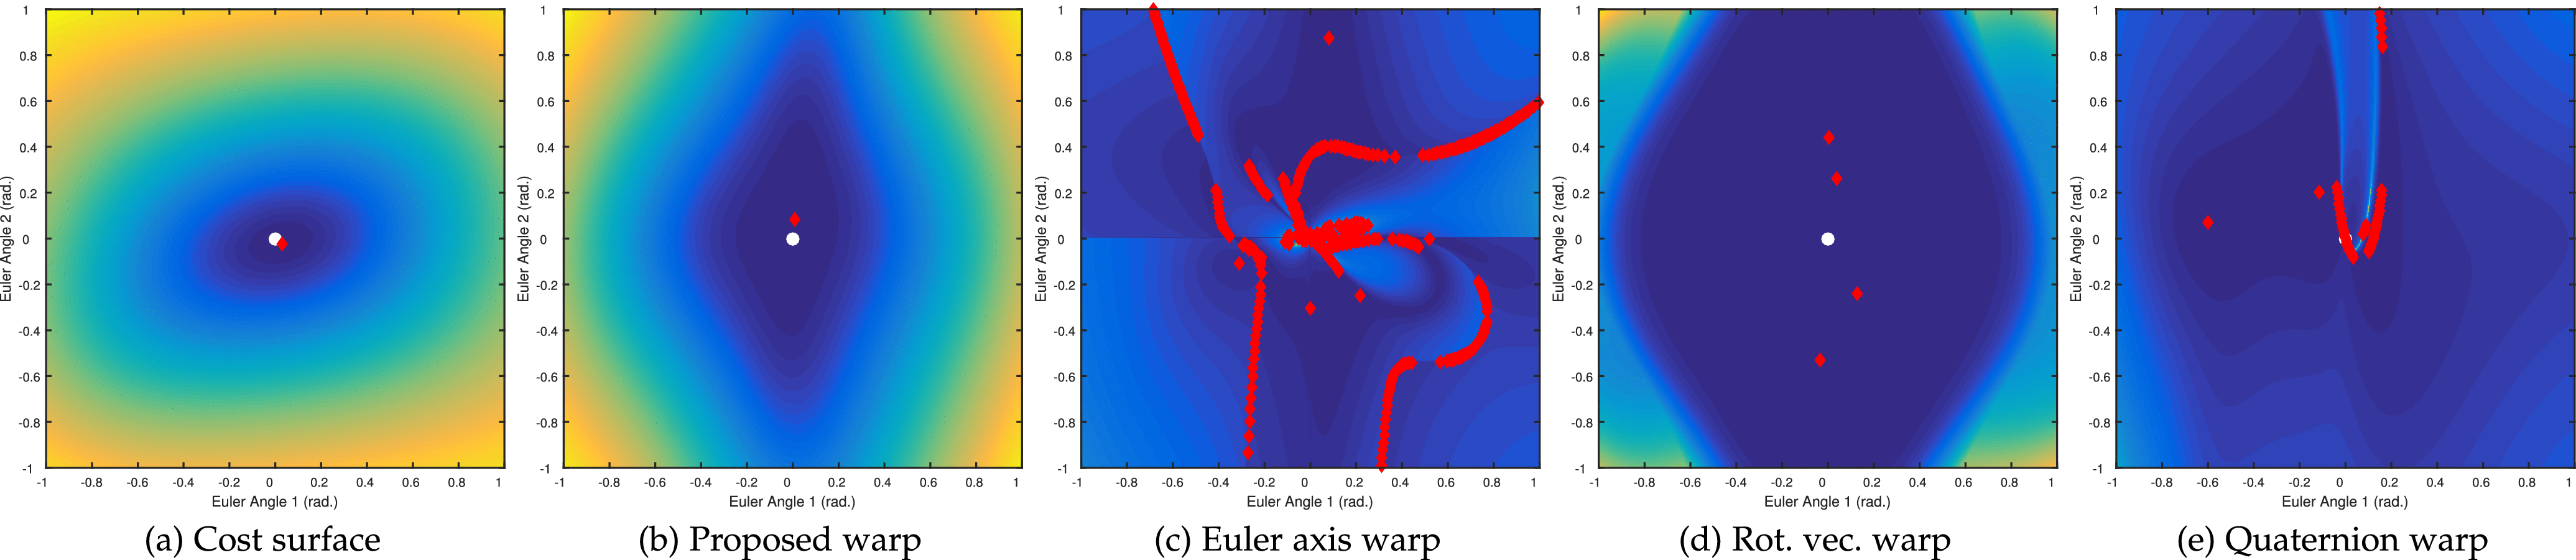
\includegraphics[scale=0.14]{hand_eye_files/vision/figures/hadfi1-2806446-hires.png}
\caption{Visualization of the PnP cost surface in the presence of noise and outliers, when optimized using different parameterizations. Color indicates the reprojection error from low (blue) to high (yellow). Fig. 1a plots this against initial camera orientation (defined by 2 Euler angles). Remaining subplots show the resulting error from a single refinement in various parameterization spaces. Diamonds indicate local minima and the white circle is the ground truth pose~\cite{8292943}. Image is made by~\cite{8292943}.}
\end{figure}
From this figure, we can clearly see
\begin{itemize}
\item Euler angles contains lots of local minima. While rotation vector shows great advantage.
\item Hybrid parameterization is more smooth.
\end{itemize}
Consequently, HARD-P$n$P formulate the objective function not only with one parameterization, but with several. They are jointly optimized via Convex Combination Descent. 

\textcolor{red}{This leaves us a new direction of how to optimize P$n$P algorithms.}


\bibliography{PnPCites} 
\bibliographystyle{ieeetr}

\end{document}